\chapter{5G architektúra}

Az 5G architektúra az ötödik generációs mobilhálózati technológia alapját képezi, amely jelentős előrelépést jelent a korábbi generációkhoz képest, mind a sebesség, mind a kapacitás és a megbízhatóság tekintetében.
Az 5G rendszer alapvetően három fő komponensből áll:

\begin{itemize}
    \item Felhasználói Berendezések (User Equipment, UE): Ezek a végfelhasználói eszközök, mint például okostelefonok, táblagépek, és más, 5G-képes eszközök, amelyek csatlakoznak a hálózathoz.
    \item Rádió Hozzáférési Hálózat (Radio Access Network, RAN): Ez a hálózati komponens biztosítja a vezeték nélküli kapcsolatot a felhasználói berendezések és a központi hálózat között.
    Az 5G RAN magába foglalja a következő elemeket:
    \begin{itemize}
        \item gNodeB (gNB): Ez az új bázisállomás, amely a rádió interfészt biztosítja a felhasználói eszközök számára.
        \item Massive MIMO és Beamforming technológiák, amelyek javítják a hálózat kapacitását és hatékonyságát.
    \end{itemize}
    \item Core Hálózat (Core Network, CN): Az 5G core hálózat a hálózat központi részét alkotja, amely az adatforgalom kezelését, a felhasználói autentikációt, és a hálózati szolgáltatások biztosítását végzi.
    Az 5G core hálózat a következő komponensekből áll:
    \begin{itemize}
        \item User Plane Function (UPF): Az adatforgalom útvonalát kezeli.
        \item Access and Mobility Management Function (AMF): A felhasználói eszközök mobilitását és hálózathoz való hozzáférését kezeli.
        \item Session Management Function (SMF): A felhasználói adatszolgáltatásokat és azok konfigurációját kezeli.
    \end{itemize}
\end{itemize}

Az 5G architektúra különlegessége, hogy támogatja a virtualizációt és a hálózati szeletelést (network slicing), amely lehetővé teszi, hogy különböző szolgáltatások és alkalmazások eltérő hálózati igényekkel különálló szeleteket kapjanak ugyanazon fizikai hálózaton belül.
Ez növeli a hálózat rugalmasságát és hatékonyságát, biztosítva a különféle felhasználói esetek, mint például az autonóm járművek, az IoT eszközök és a nagy felbontású videostreaming igényeinek kielégítését.

\section{Rádiós Hozzáférési Hálózat}

Az 5G hálózatok fizikai rétegének specifikációja a 3rd Generation Partnership Project (3GPP) nevű szervezet nevéhez kötődik.
A szervezet felelős a mobil kommunikációs hálózatok egységesítéséért, fejlesztéséért és működtetéséért.
Az új generációs ??????????

\begin{figure}[h]
    \centering
    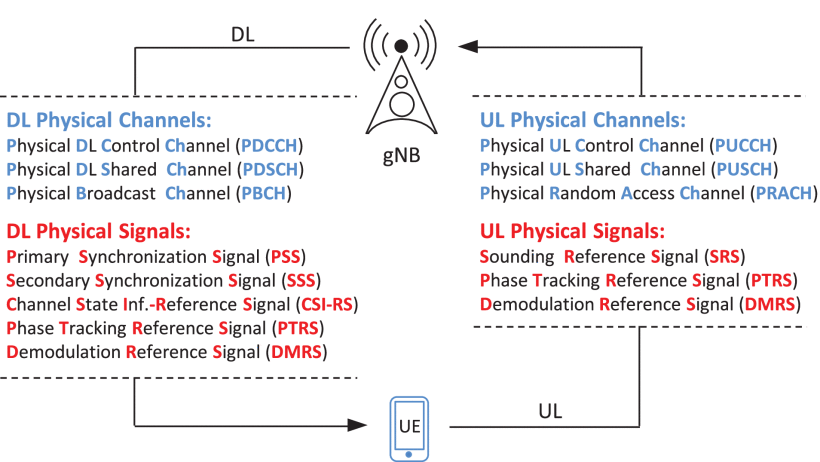
\includegraphics[width=0.6\textwidth]{jelek.png}
    \caption{Az 5G NR fizikai csatornái és jelei}
    \label{fig:jelek}
\end{figure}

\subsection{5G NR keretstruktúra}

% \begin{wrapfigure}{r}{0.38\textwidth}
%     \begin{center}
%         % \setlength{\fboxrule}{1pt}%
%         % \fboxrule=1mm
%         \fboxsep=1mm
%         \fbox{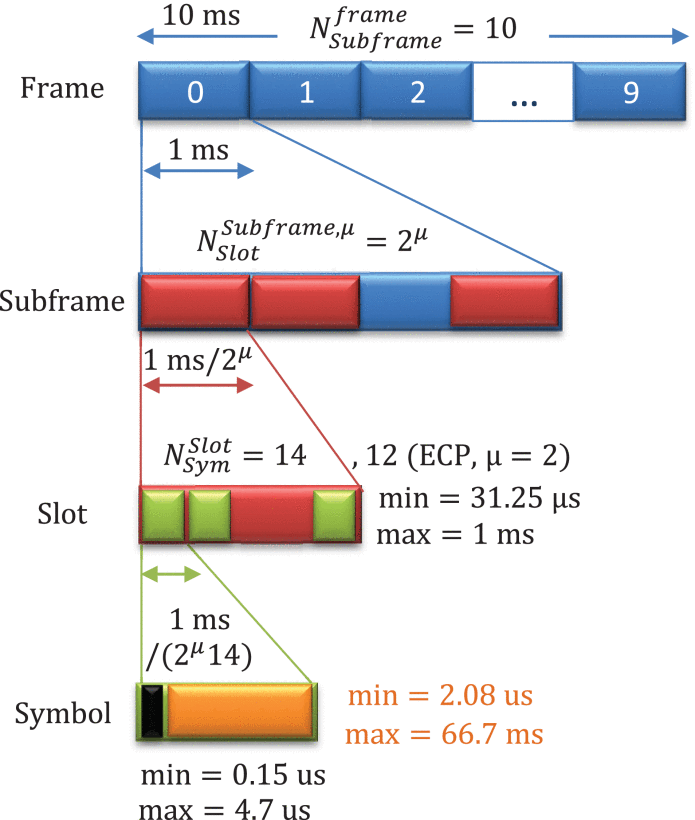
\includegraphics[width=0.36\textwidth]{slot.png}}%
%     %   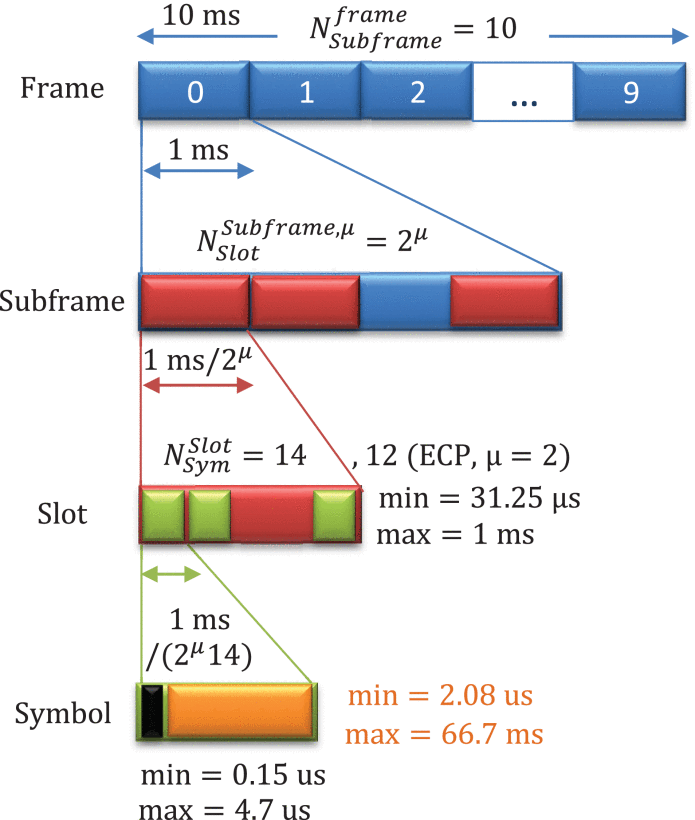
\includegraphics[width=0.38\textwidth, frame]{slot.png}
%     \end{center}
%     \caption{Birds}
%   \end{wrapfigure}

az 5G NR keretstruktúrája $N_{Subframe}^{frame}=10$ subframe-ből áll, amely közül mindegyik 1 ms idejű.
Különbség az LTE hálózatokhoz képest, hogy egy 5G NR subframe változó számú slotot tartalmaz, amelyet az alkalmazott numerológia határoz meg ($\mu$) a következő módon: $N_{Slot}^{Subframe,\mu}= 2 ^\mu$.
Ennek megfelelően egy slot időtartama $ t = \dfrac{1 \text{ ms}}{2^\mu}$.
Végezetül minden slot tartalmaz 12/14 OFDM szimbólumot attól függően, hogy normál/kiterjesztett ciklikus előtagot alkalmaz a rendszer.
Ebből következik, hogy egy OFDM szimbólum időtartama $ t = \dfrac{1 \text{ ms}}{2^\mu 12}$ vagy $ t = \dfrac{1 \text{ ms}}{2^\mu 14}$.

\begin{figure}[h!]
    \centering
    \fboxsep=1mm
    \fbox{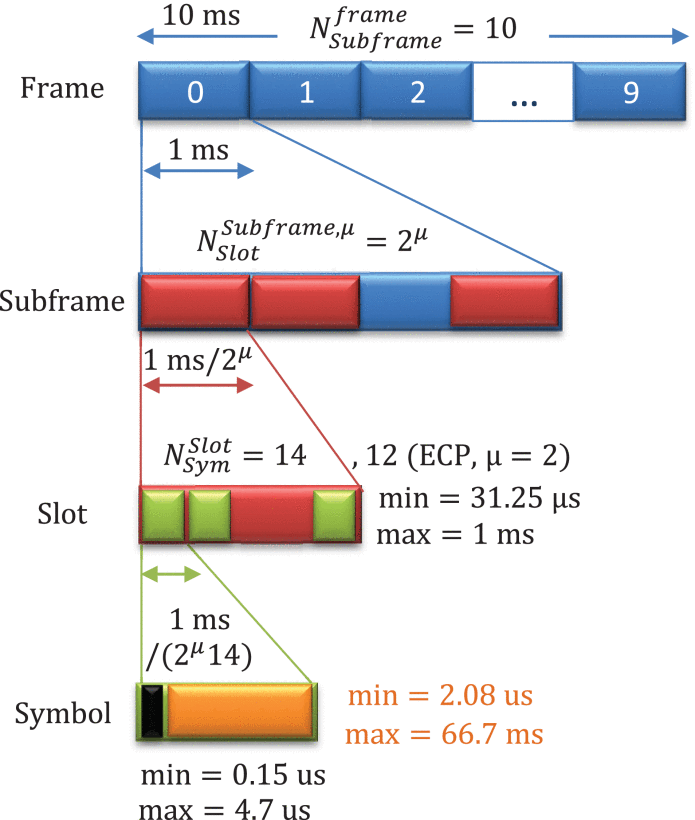
\includegraphics[width=0.4\textwidth]{slot.png}}
    % TODO: MELLÉ A KÉPLETEK
    \caption{Az 5G NR keretstruktúrája}
    \label{fig:slot}
\end{figure}



Mivel a rendszer OFDMA alapú, ezért frekvenciatartományban ún. Resource Blockokat (RB) definiál a 3GPP szabvány, mégpedig egy RB 12 egymást követő alvivőt foglal magába.
Legyen $\Delta f$ az alvivőtávolság: az 5G NR rendszerben $\Delta f$ flexibilis, és az alkalmazott numerológiától függ. $\Delta f = 15 \text{ [kHz] } 2^\mu$.


\section{Kiindulási pont}

Tekintsük az alapállapotot. Ilyenkor minden kapcsolat stabil.
Minden felhasználói készülék (User Equipment - UE) tudja, hogy milyen frekvenciacsoportban kommunikál melyik alállomással (bázisállomás).
A készülékek nem mozognakés nem történik handover.
Ebben az állapotban kapcsolunk be egy telefont.
A bekapcsoló telefon értelemszerűen elkezdi keresni a hálózatot, hogy létrejöhessen a kapcsolat, amelynek feltétele, hogy a telefon elvégezze a szinkronizációs lépéseket, és dekódolja, hogy melyik frekvenciákon kommunikálhat az alállomással.